\subsection{RQ--система с двумерным выходящим потоком} \label{section_simple_twodim}
В этом разделе будет рассмотрена модель RQ--системы, выходящий поток заявок которой, является двумерным. Другими словами, в системе обслуживаются два типа заявок --- пришедшее извне и вызванные. Исходя из этого добавим к имеющимся обозначениям следующие: \textit{$m_{1}(t)$} --- число обслуженных заявок входящего потока к моменту времени $\textit{t}$, \textit{$m_{2}(t)$} — обслуженных вызванных заявок к моменту времени $\textit{t}$.
\begin{figure}[H]
	\centering
	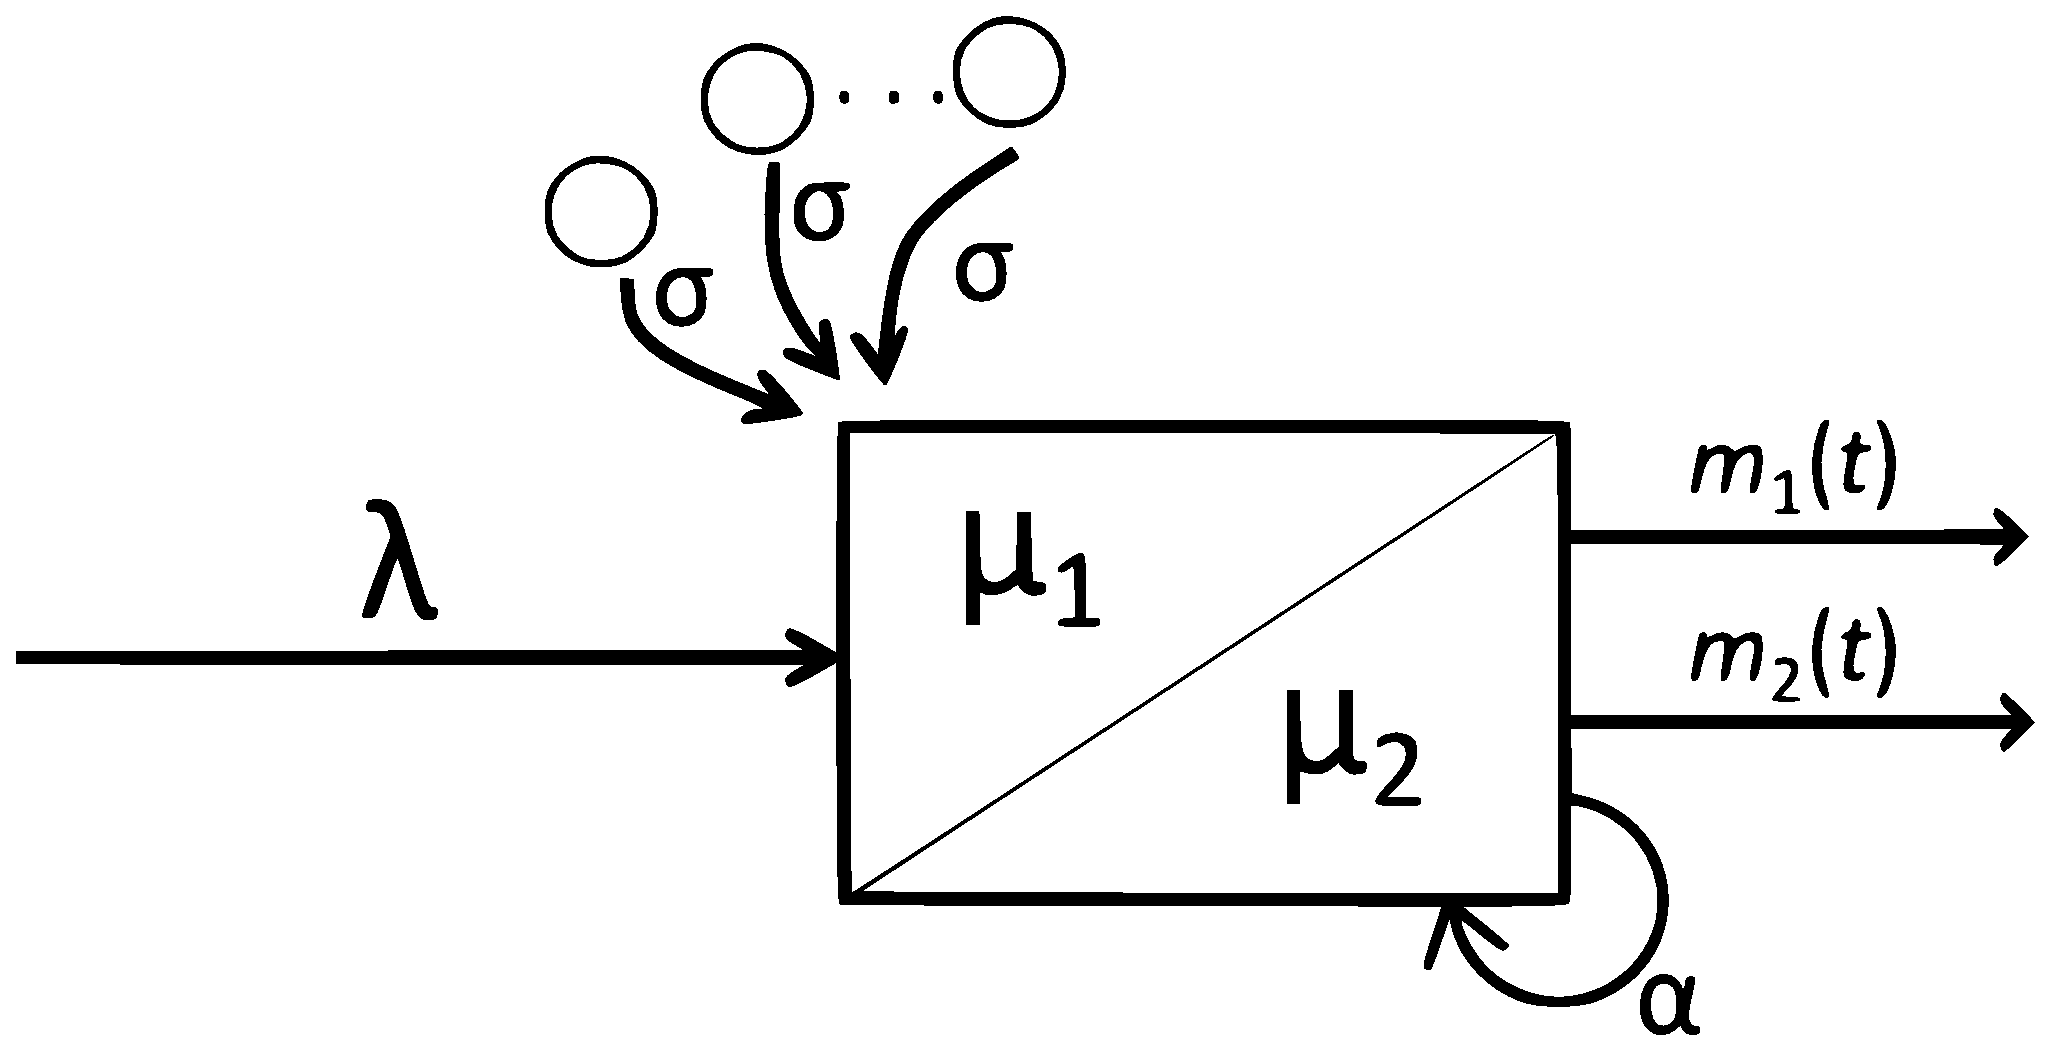
\includegraphics[scale=0.25]{twodim_output_model.eps}
	\caption{Модель RQ--системы с двумерным выходящим потоком}
	\label{twodim_output_model_fig}
\end{figure}
Функционирование данной системы аналогично рассмотренной ранее, посему процесс ее решения будет схож. 
\subsubsection{Уравнения Колмогорова}
В данном случае, мы имеем четыре характеристики, определяющие результат функционирования системы за некоторое время $t$: состояние прибора --- $\textit{k(t)}$, количество заявок на орбите --- $\textit{i(t)}$, количество обслуженных заявок входящего потока --- $m_{1}(t)$, количество обслуженных вызванных заявок --- $m_{2}(t)$,  что можно представить в виде четырех--мерного Марковского процесса
\begin{equation*}
	\{k(t),i(t),m_{1}(t),m_{2}(t)\}
\end{equation*}
Вероятность принятия прибором одного из трех состояний задается следующим образом
\begin{equation*}
	\begin{split}
		P\{k(t)=0,i(t)=i,m_{1}(t)=m_{1},m_{2}(t)=m_{2}\} &=P_{0}(i,m_{1},m_{2},t)\\
		P\{k(t)=1,i(t)=i,m_{1}(t)=m_{1},m_{2}(t)=m_{2}\} &=P_{1}(i,m_{1},m_{2},t)\\
		P\{k(t)=2,i(t)=i,m_{1}(t)=m_{1},m_{2}(t)=m_{2}\} &=P_{2}(i,m_{1},m_{2},t)
	\end{split}
\end{equation*}
Запишем систему уравнений Колмогорова, составленную на основе введенных вероятностей перехода
\begin{equation} \label{kolmogorov_equations_twodim}
	\begin{split}
		\frac{{\partial P_{0}(i,m_{1},m_{2},t)}}{{\partial t}} &= -(\lambda + i\sigma + \alpha)P_{0}(i,m_{1},m_{2},t) + P_{1}(i,m_{1}-1,m_{2},t)\mu_{1} +\\  &+ P_{2}(i,m_{1},m_{2}-1,t)\mu_{2} ,
		\\
		\frac{{\partial P_{1}(i,m_{1},m_{2},t)}}{{\partial t}} &= -(\lambda + \mu_{1})P_{1}(i,m_{1},m_{2},t) + (i+1)\sigma P_{0}(i+1,m_{1},m_{2},t) +\\ &+ \lambda  P_{0}(i,m_{1},m_{2},t),
		\\
		\frac{{\partial P_{2}(i,m_{1},m_{2},t)}}{{\partial t}} &= -(\lambda + \mu_{2})P_{2}(i,m_{1},m_{2},t) + \lambda P_{2}(i-1,m_{1},m_{2},t)  +\\ &+ \alpha  P_{0}(i,m_{1},m_{2},t).
	\end{split}
\end{equation}	
Введем частные характеристические функции, обозначив $j=\sqrt{-1}$,
\begin{equation*}
	H_{k}(u,u_{1},u_{2},t) = \sum_{i=0}^{\infty}
	\sum_{m_{1}=0}^{\infty}
	\sum_{m_{2}=0}^{\infty}  
	e^{jui}e^{ju_{1}m_{1}}e^{ju_{2}m_{2}} P_{k}(i,m_{1},m_{2},t).
\end{equation*}
Тогда перепишем систему \eqref{kolmogorov_equations_twodim} в виде
\begin{equation} \label{characteristic_equations_twodim}
	\begin{split}
		\frac{{\partial H_{0}(u,u_{1},u_{2},t)}}{{\partial t}} &= -(\lambda + \alpha)H_{0}(u,u_{1},u_{2},t) + j\sigma
		\frac{{\partial H_{0}(u,u_{1},u_{2},t)}}{{\partial u}} +\\  &+ \mu_{1} e^{ju_{1}}H_{1}(u,u_{1},u_{2},t) + \mu_{2}e^{ju_{2}}H_{2}(u,u_{1},u_{2},t) ,
		\\
		\frac{{\partial H_{1}(u,u_{1},u_{2},t)}}{{\partial t}} &= -(\lambda + \mu_{1})H_{1}(u,u_{1},u_{2},t) - j\sigma e^{-ju}
		\frac{{\partial H_{0}(u,u_{1},u_{2},t)}}{{\partial u}} +\\  &+ \lambda H_{0}(u,u_{1},u_{2},t) + \lambda e^{ju}H_{1}(u,u_{1},u_{2},t) ,
		\\
		\frac{{\partial H_{2}(u,u_{1},u_{2},t)}}{{\partial t}} &= -(\lambda + \mu_{2})H_{2}(u,u_{1},u_{2},t)  + \lambda e^{ju}H_{2}(u,u_{1},u_{2},t) +\\  &+ \alpha H_{0}(u,u_{1},u_{2},t).
	\end{split}
\end{equation}  
Бесконечное количество уравнений сведено к трем.

\subsubsection{Метод асимптотического анализа}
Полученную систему дифференциальных уравнений в частичных производных  \eqref{characteristic_equations_twodim} будем решать методом асимптотического анализа в предельном условии большой задержки заявок на орбите ($\sigma \xrightarrow{} 0$).

Обозначим $\epsilon = \sigma,   u= \epsilon w,   F_{k}(w,u_{1},u_{2},t,\epsilon) = H_{k}(u,u_{1},u_{2},t)$, тогда система запишется в виде
\begin{equation} \label{asymptotic_equations_twodim}
	\begin{split}
		\frac{{\partial F_{0}(w,u_{1},u_{2},t,\epsilon)}}{{\partial t}} &= -(\lambda + \alpha)F_{0}(w,u_{1},u_{2},t,\epsilon) + j
		\frac{{\partial F_{0}(w,u_{1},u_{2},t,\epsilon)}}{{\partial w}} +\\  &+ \mu_{1} e^{ju_{1}}F_{1}(w,u_{1},u_{2},t,\epsilon) + \mu_{2}e^{ju_{2}}F_{2}(u,u_{1},u_{2},t,\epsilon) ,
		\\
		\frac{{\partial F_{1}(w,u_{1},u_{2},t,\epsilon)}}{{\partial t}} &= -(\lambda + \mu_{1})F_{1}(w,u_{1},u_{2},t,\epsilon) - j e^{-j\epsilon w}
		\frac{{\partial F_{0}(w,u_{1},u_{2},t,\epsilon)}}{{\partial w}} +\\  &+ \lambda F_{0}(w,u_{1},u_{2},t,\epsilon) + \lambda e^{j\epsilon w}F_{1}(w,u_{1},u_{2},t,\epsilon) ,
		\\
		\frac{{\partial F_{2}(w,u_{1},u_{2},t,\epsilon)}}{{\partial t}} &= -(\lambda + \mu_{2})F_{2}(w,u_{1},u_{2},t,\epsilon)  + \lambda e^{j\epsilon w}F_{2}(w,u_{1},u_{2},t,\epsilon) +\\  &+ \alpha F_{0}(w,u_{1},u_{2},t,\epsilon).
	\end{split}
\end{equation}  
Затем, что используя условие согласованности многомерных распределений, характеристическая функция процессов $m_{1}(t$) и $m_{1}(t)$ будет записана в следующем виде с введенными функциями 
\begin{equation*}
	M\{\exp(ju_{1}m_{1}(t))\exp(ju_{2}m_{2}(t))\}=\sum_{k=0}^{2}H_{k}(0,u_{1},u_{2},t) = \sum_{k=0}^{2}F_{k}(0,u_{1},u_{2},t,\epsilon).
\end{equation*}

\begin{theorem}
	Асимптотические приближение двумерной характеристической функции числа обслуженных заявок входящего потока и числа обслуженных вызванных заявок за некоторое время $t$ имеет вид
	\begin{equation*} \label{theorem_twodim}
		\begin{split}
			\boldsymbol{F}(u_{1},u_{2},t) =  \lim_{\sigma \xrightarrow{} 0} M\{\exp(ju_{1}m_{1}(t))\exp(ju_{2}m_{2}(t))\} &= 
			\\
			= \lim_{\epsilon \xrightarrow{} 0} \sum_{k=0}^{2}F_{k}(0,u_{1},u_{2},t,\epsilon) = \boldsymbol{R} \cdot \exp\{G(u_{1},u_{2})t\} \cdot \boldsymbol{E}
		\end{split}
	\end{equation*}
	где 
	\begin{equation*}
		\boldsymbol{G}(u_{1},u_{2})=\begin{bmatrix}
			-(\lambda + \alpha + \kappa) & \mu_{1}e^{ju_{1}} &  \mu_{2}e^{ju_{2}}\\
			\kappa+\lambda & -\mu_{1} & 0\\
			\alpha & 	0 &	-\mu_{2}
		\end{bmatrix}^{T},
	\end{equation*}
	вектор--строка $\boldsymbol{R}=\{R_{0},R_{1},R_{2}\}$ --- стационарное распределение вероятности состояния прибора
	\begin{equation*}
		\boldsymbol{R}=\{\frac{\mu_{2}(\mu_{1} - \lambda)}{\mu_{1}(\mu_{2} - \alpha)},\frac{\lambda}{\mu_{1}},\frac{\alpha(\mu_{1} - \lambda)}{\mu_{1}(\mu_{2} + \alpha)}\},
	\end{equation*}
	$\kappa$ --- нормированное среднее число заявок на орбите
	\begin{equation*}
		\kappa = \frac{\lambda(\lambda \mu_{2} + \alpha \mu_{1})}{\mu_{2}(\mu_{1} - \lambda)},
	\end{equation*}
	а $\boldsymbol{E}$ --- единичный вектор--столбец соответствующей размерности.
\end{theorem}
\begin{proof}
	Делая предельный переход $ \lim_{\epsilon \xrightarrow{} 0} F_{k}(w,u_{1},u_{2},t,\epsilon) = F_{k}(w,u_{1},u_{2},t)$  в полученной системе \eqref{asymptotic_equations_twodim} , система уравнений будет записана в виде
	\begin{equation} \label{eps_limit_twodim}
		\begin{split}
			\frac{{\partial F_{0}(w,u_{1},u_{2},t)}}{{\partial t}} &= -(\lambda + \alpha)F_{0}(w,u_{1},u_{2},t) + j
			\frac{{\partial F_{0}(w,u_{1},u_{2},t)}}{{\partial w}} +\\  &+ \mu_{1} e^{ju_{1}}F_{1}(w,u_{1},u_{2},t) + \mu_{2}e^{ju_{2}}F_{2}(w,u_{1},u_{2},t) ,
			\\
			\frac{{\partial F_{1}(w,u_{1},u_{2},t)}}{{\partial t}} &= -(\lambda + \mu_{1})F_{1}(w,u_{1},u_{2},t) - j 
			\frac{{\partial F_{0}(w,u_{1},u_{2},t)}}{{\partial w}} +\\  &+ \lambda F_{0}(w,u_{1},u_{2},t) + \lambda F_{1}(w,u_{1},u_{2},t) ,
			\\
			\frac{{\partial F_{2}(w,u_{1},u_{2},t)}}{{\partial t}} &= -(\lambda + \mu_{2})F_{2}(w,u_{1},u_{2},t)  + \lambda F_{2}(w,u_{1},u_{2},t) +\\  &+ \alpha F_{0}(w,u_{1},u_{2},t).
		\end{split}
	\end{equation}  
	Решение системы \eqref{eps_limit_twodim} будет получено в следующей форме
	\begin{equation} \label{solution_twodim}
		F_{k}(w,u_{1},u_{2},t) = \Phi(w)F_{k}(u_{1},u_{2},t).
	\end{equation}  
	$\Phi(w)$ --- асимптотическое приближение характеристической функции числа заявок на орбите при условии большой задержки на орбите.
	
	Подставив \eqref{solution_twodim} в систему \eqref{eps_limit_twodim} и разделив обе части уравнений на $\Phi(w)$, получим
	\begin{equation} \label{preresult_twodim}
		\begin{split}
			\frac{{\partial F_{0}(u_{1},u_{2},t)}}{{\partial t}} &= -(\lambda + \alpha)F_{0}(u_{1},u_{2},t) + j
			\frac{\Phi'(w) }{\Phi(w)}F_{0}(u_{1},u_{2},t) +\\  &+ \mu_{1} e^{ju_{1}}F_{1}(u_{1},u_{2},t) + \mu_{2}e^{ju_{2}}F_{2}(u_{1},u_{2},t) ,
			\\
			\frac{{\partial F_{1}(u_{1},u_{2},t)}}{{\partial t}} &= -(\lambda + \mu_{1})F_{1}(u_{1},u_{2},t) - j 
			\frac{\Phi'(w) }{\Phi(w)}F_{0}(u_{1},u_{2},t) +\\  &+ \lambda F_{0}(u_{1},u_{2},t) + \lambda F_{1}(u_{1},u_{2},t) ,
			\\
			\frac{{\partial F_{2}(u_{1},u_{2},t)}}{{\partial t}} &= -(\lambda + \mu_{2})F_{2}(u_{1},u_{2},t)  + \lambda F_{2}(u_{1},u_{2},t) +\\  &+ \alpha F_{0}(u_{1},u_{2},t).
		\end{split}
	\end{equation}  
	%Заметим, что $w$ содержится только в отношении $\frac{\Phi'(w) }{\Phi(w)}$, а остальные слагаемые и левые части уравнений не зависят от $w$. Это означает, что  $\Phi(w)$ имеет вид экспоненты. Учитывая, что  $\Phi(w)$ имеет смысл асимптотического приближения характеристической функции числа заявок на орбите, мы можем конкретизировать вид данной функции
	%\begin{equation*}
	%	\frac{\Phi'(w) }{\Phi(w)} = \frac{e^{j\kappa w}j\kappa}{e^{j\kappa w}},
	%\end{equation*} 
	%где $\kappa$ - нормированное среднее число заявок на орбите, которое было получено в %\cite{nazarov2017asymptotic} и имеет вид 
	%\begin{equation*}
%		\kappa = \frac{\lambda(\lambda \mu_{2} + \alpha \mu_{1})}{\mu_{2}(\mu_{1} - \lambda)}.
%	\end{equation*}
	Ранее, мы конкретизировали вид $\Phi(w)$ в \eqref{Phi_concrete}, что позволяет нам привести систему \eqref{preresult_twodim} к следующему виду	
	\begin{equation} \label{result_twodim}
		\begin{split}
			\frac{{\partial F_{0}(u_{1},u_{2},t)}}{{\partial t}} &= -(\lambda + \alpha+ \kappa)F_{0}(u_{1},u_{2},t) + \\  &+ \mu_{1} e^{ju_{1}}F_{1}(u_{1},u_{2},t) + \mu_{2}e^{ju_{2}}F_{2}(u_{1},u_{2},t) ,
			\\
			\frac{{\partial F_{1}(u_{1},u_{2},t)}}{{\partial t}} &= (\lambda + \kappa)F_{0}(u_{1},u_{2},t) -  
			\mu_{1}F_{1}(u_{1},u_{2},t) +\\  &+  0F_{2}(u_{1},u_{2},t) ,
			\\
			\frac{{\partial F_{2}(u_{1},u_{2},t)}}{{\partial t}} &= \alpha F_{0}(u_{1},u_{2},t)   +  0F_{1}(u_{1},u_{2},t) -\\  &- \mu_{2}F_{2}(u_{1},u_{2},t).
		\end{split}
	\end{equation}  
	Введем следующие обозначения
	\begin{equation*}
		\boldsymbol{F}(u_{1},u_{2},t) = \{F_{0}(u_{1},u_{2},t),F_{1}(u_{1},u_{2},t),F_{1}(u_{2},u_{2},t)\},
	\end{equation*}  
	\begin{equation*}
		\boldsymbol{G}(u_{1},u_{2})=\begin{bmatrix}
			-(\lambda + \alpha + \kappa) & \mu_{1}e^{ju_{1}} &  \mu_{2}e^{ju_{2}}\\
			\kappa+\lambda & -\mu_{1} & 0\\
			\alpha & 	0 &	-\mu_{2}
		\end{bmatrix}^{T},
	\end{equation*}
	$\boldsymbol{G}(u_{1},u_{2})$ --- транспонированная матрица коэффициентов системы \eqref{result_twodim}.
	Тогда получим следующее матричное уравнение
	\begin{equation*}
		\frac{{\partial \boldsymbol{F}(u_{1},u_{2},t)}}{{\partial t}} =\boldsymbol{F}(u_{1},u_{2},t)\boldsymbol{G}(u_{1},u_{2}),
	\end{equation*}
	общее решение которого имеет вид
	\begin{equation} \label{diff_twodim}
		\boldsymbol{F}(u_{1},u_{2},t)=\boldsymbol{C}e^{\boldsymbol{G}(u_{1},u_{2})t}.
	\end{equation}
	Для получения единственного решения примем в рассмотрение начальное условие
	\begin{equation} \label{cauchi_condition_twodim}
		\boldsymbol{F}(u_{1},u_{2},0)=\boldsymbol{R},
	\end{equation}
	где вектор--строка $\boldsymbol{R}$ --- стационарное распределение вероятности состояния прибора, то есть процесса $k(t)$, которое имеет форму \cite{nazarov2017asymptotic}
	\begin{equation*}
		\boldsymbol{R}=\{\frac{\mu_{2}(\mu_{1} - \lambda)}{\mu_{1}(\mu_{2} - \alpha)},\frac{\lambda}{\mu_{1}},\frac{\alpha(\mu_{1} - \lambda)}{\mu_{1}(\mu_{2} + \alpha)}\}.
	\end{equation*}
	Описав начальное условие, переходим к решению задачи Коши (\ref{diff_twodim}, \ref{cauchi_condition_twodim}).
	
	Чтобы получить маргинальное распределение вероятностей числа обслуженных заявок, суммируем компоненты вектор--строки $\boldsymbol{F}(u_{1},u_{2},t)$ по $k$ и умножаем результат на единичный вектор--столбец $\boldsymbol{E}$. Получим
	\begin{equation}\label{approximation_twodim}
		\boldsymbol{F}(u_{1},u_{2},t)\boldsymbol{E}=\boldsymbol{R}e^{\boldsymbol{G}(u_{1},u_{2})t}\boldsymbol{E}.
	\end{equation}
	Формула \eqref{approximation_twodim} является решением рассматриваемой системы. 
\end{proof}

\subsubsection{Переход к явному распределению вероятностей} \label{distr_find_twodim}
Характеристическая функция \eqref{approximation_twodim} описывает процессы $m_{1}(t)$ и $m_{2}(t)$, однако делает это в неявной форме. Для использования полученной формулы для расчетов, получим явное распределение вероятностей.
Формула \eqref{approximation_twodim}, так же как и \eqref{approximation_summary} содержит матричную экспоненту, к которой мы применим преобразование подобия \cite{bronson1991matrix}
\begin{equation*}
	\boldsymbol{G}(u_{1},u_{2}) =\boldsymbol{T}(u_{1},u_{2})\boldsymbol{GJ}(u_{1},u_{2})\boldsymbol{T}(u_{1},u_{2})^{-1},
\end{equation*}
где $\boldsymbol{T}(u_{1},u_{2})$ – матрицы собственных вектором матрицы $\boldsymbol{G}(u_{1},u_{2})$, а $\boldsymbol{GJ}(u_{1},u_{2})$ --- диагональная матрицы, содержащая собственные числа $\boldsymbol{G}(u_{1},u_{2})$. Данное преобразование справедливо для любой степени $m$ некоторой матрицы $\boldsymbol{A}^{m}$, из чего следует, что оно так же справедливо для матричной экспоненты \cite{egorov2006prog}
\begin{equation*}
	e^{\boldsymbol{G}(u_{1},u_{2})t}=\boldsymbol{T}(u_{1},u_{2})\cdot \begin{bmatrix}
		e^{t \Lambda_{1}(u_{1},u_{2})} & 0 &  0\\
		0 & e^{t \Lambda_{2}(u_{1},u_{2})} & 0\\
		0 & 0 &	e^{t \Lambda_{3}(u_{1},u_{2})}
	\end{bmatrix} \cdot \boldsymbol{T}(u_{1},u_{2})^{-1},
\end{equation*}
где $\Lambda_{n}$ --- собственное число матрицы $\boldsymbol{G}(u_{1},u_{2})$. Тогда распределение примет следующий вид
\begin{equation*}
	\boldsymbol{F}(u_{1},u_{2},t)=\boldsymbol{R} \cdot \boldsymbol{T}(u_{1},u_{2})\cdot \begin{bmatrix}
		e^{t \Lambda_{1}(u_{1},u_{2})} & 0 &  0\\
		0 & e^{t \Lambda_{2}(u_{1},u_{2})} & 0\\
		0 & 0 &	e^{t \Lambda_{3}(u_{1},u_{2})}
	\end{bmatrix} \cdot \boldsymbol{T}(u_{1},u_{2})^{-1} \cdot \boldsymbol{E}.
\end{equation*}
Для восстановления распределения используем обратное преобразование Фурье для дискретных величин
\begin{equation} \label{distr_simple_twodim}
	P(m_{1},m_{2},t) = \dfrac{1}{2\pi}\int_{-\pi}^{\pi}\int_{-\pi}^{\pi} e^{-i \cdot u_{1} \cdot m_{1}} e^{-i \cdot u_{2} \cdot m_{2}}\boldsymbol{F}(u_{1},u_{2},t)du_{2}du_{2}.
\end{equation}
Полученная формула характеризует вероятность обслуживания $m_{1}$ входящих заявок и $m_{2}$ вызванных заявок к моменту времени $t$ в рассматриваемой системе.

\subsubsection{Коэффициент корреляции} \label{corr_section}
Полученное асимптотические приближение характеристической функции \eqref{approximation_twodim} позволяет нам подробнее изучить выходящие потоки рассматриваемой системы, а именно --- найти корреляционную зависимость случайных процессов $m_{1}(t)$ и $m_{2}(t)$.
Рассмотрим нахождение коэффициента корреляции, который будет зависеть от параметра $t$
\begin{equation*}
	r(t) = \frac{\textnormal{cov}(m_{1}(t),m_{2}(t))}{\sqrt{D(m_{1}(t))}\sqrt{D(m_{2}(t))}}.
\end{equation*}
Воспользуемся свойством характеристической функции о существовании ее $n$--ой производной, соответствующей $n$--му начальному моменту случайной величины. Тогда ковариация и дисперсия будут вычисляться следующим образом
\begin{equation*}
	\begin{split}
		\textnormal{cov}(m_{1}(t),m_{2}(t)) &= M\{m_{1}(t)m_{2}(t)\} - M\{m_{1}(t)\}M\{m_{2}(t)\} = \frac{1}{j^{2}}\frac{{\partial}^{2}}{{\partial u_{1}}{\partial u_{2}}}\boldsymbol{F}(u_{1},u_{2},t) \bigg\rvert_{\substack{u_{1} = 0 \\ u_{2} = 0}} - \\ &- \frac{1}{j^{2}} \frac{{\partial}}{{\partial u_{1}}} \boldsymbol{F}(u_{1},u_{2},t) \bigg\rvert_{\substack{u_{1} = 0 \\ u_{2} = 0}} \frac{{\partial}}{{\partial u_{2}}} \boldsymbol{F}(u_{1},u_{2},t) \bigg\rvert_{\substack{u_{1} = 0 \\ u_{2} = 0}},
		\\
		D\{m_{1}(t)\} &= M^{2}\{m_{1}(t)\} - (M\{m_{1}(t)\})^{2} = \frac{1}{j^{2}}\frac{{\partial}^{2}}{{\partial u_{1}}^{2}}\boldsymbol{F}(u_{1},u_{2},t) \bigg\rvert_{\substack{u_{1} = 0 \\ u_{2} = 0}}  - \\ &- (\frac{1}{j^{2}} \frac{{\partial}}{{\partial u_{1}}} \boldsymbol{F}(u_{1},u_{2},t) \bigg\rvert_{\substack{u_{1} = 0 \\ u_{2} = 0}})^{2},
		\\
		D\{m_{2}(t)\} &= M^{2}\{m_{2}(t)\} - (M\{m_{2}(t)\})^{2} = \frac{1}{j^{2}}\frac{{\partial}^{2}}{{\partial u_{2}}^{2}}\boldsymbol{F}(u_{1},u_{2},t) \bigg\rvert_{\substack{u_{1} = 0 \\ u_{2} = 0}}  - \\ &- (\frac{1}{j^{2}} \frac{{\partial}}{{\partial u_{2}}} \boldsymbol{F}(u_{1},u_{2},t) \bigg\rvert_{\substack{u_{1} = 0 \\ u_{2} = 0}})^{2}.
	\end{split}
\end{equation*}
Полученные формулы позволяют использовать нам численно исследовать поведение системы при разных параметрах.
\clearpage